\documentclass[12pt, A4]{article}

% Packages
	% Basics
		\usepackage{amsmath}
		\usepackage{bm}
		\usepackage{cellspace}
		\usepackage{csquotes}
		\usepackage[shortlabels]{enumitem}
		\usepackage[hang,flushmargin]{footmisc}
		\usepackage[margin=0.75in]{geometry}
		\usepackage{hyperref}
		\usepackage[utf8]{inputenc}
		\usepackage{kbordermatrix}
	% Diagrams
		\usepackage{pgfplots}
		\usepackage{tikz}
		\usepackage{tikz-3dplot}
			\usetikzlibrary{arrows,decorations.markings,plotmarks}
	% Formatting
		\usepackage{booktabs}
		\usepackage{tasks}
	% Symbols
		\usepackage{amssymb} % Miscellaneous
		\usepackage{esint} % Integrals
		\usepackage{physics} % Differentials
% Configuration
	\title{Homework Set 2}
	\author{Arnav Patri}
	\hypersetup{
	    colorlinks,
	    citecolor=black,
	    filecolor=black,
	    linkcolor=black,
	    urlcolor=black
	}
	\cellspacetoplimit10pt
	\cellspacebottomlimit10pt
	
% Macros
	% Notation
		% Matrices
			\newcommand{\lmatrix}[2]{
				\begin{array}{cc}
					& #1 \\
					#1 & #2
				\end{array}
			}
		% Operators
			\DeclareMathOperator{\divr}{div}
		% Sets
			\newcommand{\R}{\mathbb{R}}
		% Other
			\DeclareMathOperator{\avg}{avg}
			\DeclareMathOperator{\return}{\text{return}}
			\renewcommand{\th}{\text{th}}
			\DeclareMathOperator{\while}{\text{while}}
	% Utilities
		\newcommand{\callout}[2]{\begin{center}\fbox{\begin{minipage}{#1cm}#2\end{minipage}}\end{center}}
		\newcommand{\comment}[1]{}
		\newcommand{\enumset}[1]{\setcounter{enumi}{#1}}
		\newcommand{\subsectionb}[1]{\subsection*{#1}\addcontentsline{toc}{subsection}{#1}}	

\begin{document}
	\maketitle
	
	\setcounter{section}{9}
	\section{Graphs}
		\subsection{Graphs and Graph Models}
			\begin{enumerate}
				\enumset{2}
				\item
					The graph has undirected edges and no loops, making it a simple graph.
				\item
					The graph has multiple undirected edges and no loops, making it a multigraph.
				\item
					The graph has multiple undirected edges and loops, making it a psuedograph.
				\item
					The graph has multiple undirected edges and no loops, making it a multigraph.
				\item
					The graph has directed edges and loops, making it a digraph.
				\item
					The graph has multiple directed edges and loops, making it a directed multigraph.
				\item
					The graph has multiple directed edges and loops, making it a directed multigraph.
			\end{enumerate}
		\subsection{Graph Terminology and Special Types of Graphs}
			\begin{enumerate}
				\item
					\(|V| = 6\), \(|E| = 6\), \(\deg a = 2\) , \(\deg b = 4\), \(\deg c = 1\) (pendant), \(\deg d = 0\) (isolated), \(\deg e = 2\), \(\deg f = 3\)
				\item
					\(|V| = 5\), \(|E| = 13\), \(\deg a = 6\), \(\deg b = 6\), \(\deg c = 6\), \(\deg d = 5\), \(\deg e = 3\)
				\item
					\(|V| = 9\), \(|E| = 12\), \(\deg a = 3\), \(\deg b = 2\), \(\deg c = 4\), \(\deg d = 0\) (isolated), \(\deg e = 6\), \(\deg f = 0\) (isolated), \(\deg g = 4\), \(\deg h = 2\), \(\deg i = 3\)
				\enumset{4}
				\item
					A simple graph with 15 vertices each of degree 5 cannot exist, as all graphs must have an even number of vertices of odd degree.
				\enumset{6}
				\item
					\(|V| = 4\), \(E = 7\), \(\deg^-a = 3\), \(\deg^+a = 1\), \(\deg^-b = 1\), \(\deg^+b = 2\), \(\deg^-c = 2\), \(\deg^+c = 1\), \(\deg^-d = 1\), \(\deg^+d = 3\)
				\item
					\(|V| = 4\), \(|E| = 8\), \(\deg^-a = 1\), \(\deg^-b = 3\), \(\deg^-c = 2\), \(\deg^-d = 1\), \(\deg^+a = 2\), \(\deg^+b = 4\), \(\deg^+c = 1\), \(\deg^+d = 1\)
				\item
					\(|V| = 5\), \(E = 13\), \(\deg^-a = 6\), \(\deg^+a = 1\), \(\deg^-b = 1\), \(\deg^=b = 5\), \(\deg^-c = 2\), \(\deg^+c = 5\), \(\deg^-d = 4\), \(\deg^=d = 2\), \(\deg^- e = 0\), \(\deg^=e = 0\)
				\enumset{19}
				\item
					\begin{tasks}(3)
						\task
							\[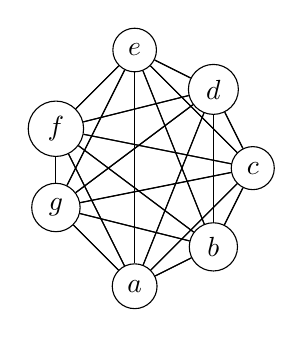
\begin{tikzpicture}
								\node[circle, draw] (a1) at (0, 0) {\(a\)};
								\node[circle, draw] (a2) at (1, 0.5) {\(b\)};
								\node[circle, draw] (a3) at (1.5, 1.5) {\(c\)};
								\node[circle, draw] (a4) at (1, 2.5) {\(d\)};
								\node[circle, draw] (a5) at (0, 3) {\(e\)};
								\node[circle, draw] (a6) at (-1, 2) {\(f\)};
								\node[circle, draw] (a7) at (-1, 1){\(g\)};
								\foreach \x in {1,...,7}
									\foreach \y in {1,...,7}
										\draw (a\x) -- (a\y);
							\end{tikzpicture}\]
						\task
							\[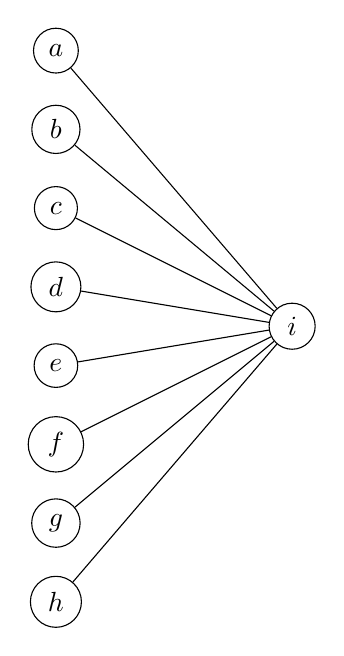
\begin{tikzpicture}
								\node[circle, draw] (a1) at (0, 0) {\(a\)};
								\node[circle, draw] (a2) at (0, -1) {\(b\)}; 
								\node[circle, draw] (a3) at (0, -2) {\(c\)};
								\node[circle, draw] (a4) at (0, -3) {\(d\)};
								\node[circle, draw] (a5) at (0, -4) {\(e\)};
								\node[circle, draw] (a6) at (0, -5) {\(f\)};
								\node[circle, draw] (a7) at (0, -6) {\(g\)};
								\node[circle, draw] (a8) at (0, -7) {\(h\)};
								\node[circle, draw] (a9) at (3, -3.5) {\(i\)};
								\foreach \x in {1,...,8}
									\draw (a\x) -- (a9);
							\end{tikzpicture}\]
						\task
							\[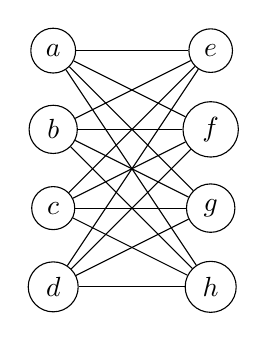
\begin{tikzpicture}
								\node[circle, draw] (a1) at (0, 0) {\(a\)};
								\node[circle, draw] (a2) at (0, -1) {\(b\)};
								\node[circle, draw] (a3) at (0, -2) {\(c\)};
								\node[circle, draw] (a4) at (0, -3) {\(d\)};
								\node[circle, draw] (a5) at (2, 0) {\(e\)};
								\node[circle, draw] (a6) at (2, -1) {\(f\)};
								\node[circle, draw] (a7) at (2, -2) {\(g\)};
								\node[circle, draw] (a8) at (2, -3) {\(h\)};
								\foreach \x in {1,...,4}
									\foreach \y in {5,...,8}
										\draw (a\x) -- (a\y);
							\end{tikzpicture}\]
						\task
							\[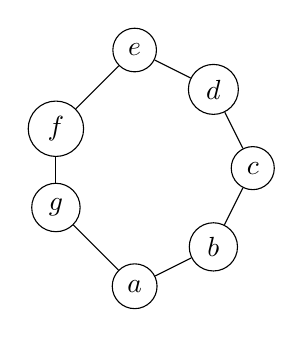
\begin{tikzpicture}
								\node[circle, draw] (a1) at (0, 0) {\(a\)};
								\node[circle, draw] (a2) at (1, 0.5) {\(b\)};
								\node[circle, draw] (a3) at (1.5, 1.5) {\(c\)};
								\node[circle, draw] (a4) at (1, 2.5) {\(d\)};
								\node[circle, draw] (a5) at (0, 3) {\(e\)};
								\node[circle, draw] (a6) at (-1, 2) {\(f\)};
								\node[circle, draw] (a7) at (-1, 1){\(g\)};
								\draw (a1) -- (a2);
								\draw (a2) -- (a3);
								\draw (a3) -- (a4);
								\draw (a4) -- (a5);
								\draw (a5) -- (a6);
								\draw (a6) -- (a7);
								\draw (a7) -- (a1);
							\end{tikzpicture}\]
						\task
							\[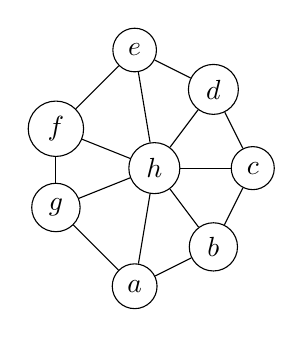
\begin{tikzpicture}
								\node[circle, draw] (a1) at (0, 0) {\(a\)};
								\node[circle, draw] (a2) at (1, 0.5) {\(b\)};
								\node[circle, draw] (a3) at (1.5, 1.5) {\(c\)};
								\node[circle, draw] (a4) at (1, 2.5) {\(d\)};
								\node[circle, draw] (a5) at (0, 3) {\(e\)};
								\node[circle, draw] (a6) at (-1, 2) {\(f\)};
								\node[circle, draw] (a7) at (-1, 1){\(g\)};
								\node[circle, draw] (a8) at (0.25, 1.5) {\(h\)};
								\draw (a1) -- (a2);
								\draw (a2) -- (a3);
								\draw (a3) -- (a4);
								\draw (a4) -- (a5);
								\draw (a5) -- (a6);
								\draw (a6) -- (a7);
								\draw (a7) -- (a1);
								\foreach \x in {1,...,7}
									\draw (a\x) -- (a8);
							\end{tikzpicture}\]
						\task
							
					\end{tasks}
				\item
					\[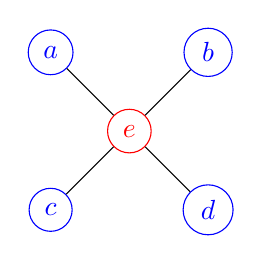
\begin{tikzpicture}
						\node[circle, draw, blue] (a) at (-1, 1) {\(a\)};
						\node[circle, draw, blue] (b) at (1, 1) {\(b\)};
						\node[circle, draw, blue] (c) at (-1, -1) {\(c\)};
						\node[circle, draw, blue] (d) at (1, -1) {\(d\)};
						\node[circle, draw, red] (e) at (0, 0) {\(e\)};
						\draw (a) -- (e) -- (d);
						\draw (c) -- (e) -- (b);
					\end{tikzpicture}\]
					The graph is bipartite.
				\item
					\[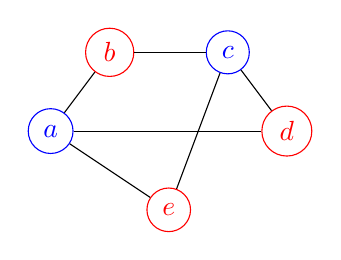
\begin{tikzpicture}
						\node[circle, draw, blue] (a) at (-1.5, 0) {\(a\)};
						\node[circle, draw, red] (b) at (-0.75, 1) {\(b\)};
						\node[circle, draw, blue] (c) at (0.75, 1) {\(c\)};
						\node[circle, draw, red] (d) at (1.5, 0) {\(d\)};
						\node[circle, draw, red] (e) at (0, -1) {\(e\)};
						\draw (a) -- (b);
						\draw (a) -- (d);
						\draw (a) -- (e);
						\draw (b) -- (c);
						\draw (c) -- (d);
						\draw (c) -- (e);
					\end{tikzpicture}\]
					The graph is bipartite.
				\item
					\[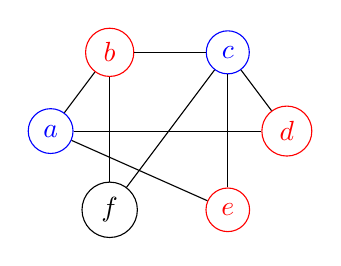
\begin{tikzpicture}
						\node[circle, draw, blue] (a) at (-1.5, 0) {\(a\)};
						\node[circle, draw, red] (b) at (-0.75, 1) {\(b\)};
						\node[circle, draw, blue] (c) at (0.75, 1) {\(c\)};
						\node[circle, draw, red] (d) at (1.5, 0) {\(d\)};
						\node[circle, draw, red] (e) at (0.75, -1) {\(e\)};
						\node[circle, draw] (f) at (-0.75, -1) {\(f\)};
						\draw (a) -- (b);
						\draw (a) -- (d);
						\draw (a) -- (e);
						\draw (b) -- (c);
						\draw (b) -- (f);
						\draw (c) -- (d);
						\draw (c) -- (e);
						\draw (c) -- (f);
					\end{tikzpicture}\]
					This graph is not bipartite, due to \(f\).
				\item
					\[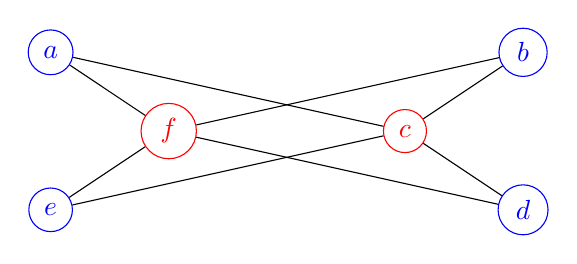
\begin{tikzpicture}
						\node[circle, draw, blue] (a) at (-3, 1) {\(a\)};
						\node[circle, draw, blue] (b) at (3, 1) {\(b\)};
						\node[circle, draw, red] (c) at (1.5, 0) {\(c\)};
						\node[circle, draw, blue] (d) at (3, -1) {\(d\)};
						\node[circle, draw, blue] (e) at (-3, -1) {\(e\)};
						\node[circle, draw, red] (f) at (-1.5, 0) {\(f\)};
						\draw (a) -- (c);
						\draw (a) -- (f);
						\draw (b) -- (f);
						\draw (b) -- (c);
						\draw (c) -- (d);
						\draw (c) -- (e);
						\draw (d) -- (f);
						\draw (e) -- (f);
					\end{tikzpicture}\]
					This graph is bipartite.
				\item
					\[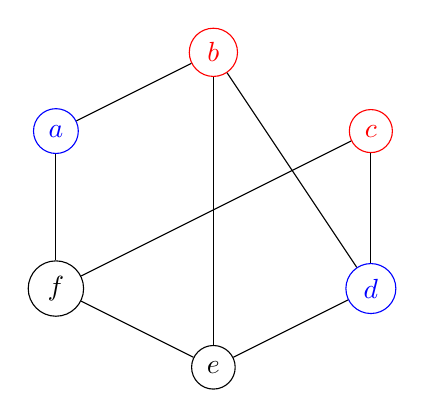
\begin{tikzpicture}
						\node[circle, draw, blue] (a) at (-2, 2) {\(a\)};
						\node[circle, draw, red] (b) at (0, 3) {\(b\)};
						\node[circle, draw, red] (c) at (2, 2) {\(c\)};
						\node[circle, draw, blue] (d) at (2, 0) {\(d\)};
						\node[circle, draw] (e) at (0, -1) {\(e\)};
						\node[circle, draw] (f) at (-2, 0) {\(f\)};
						\draw (a) -- (b);
						\draw (a) -- (f);
						\draw (b) -- (d);
						\draw (b) -- (e);
						\draw (c) -- (d);
						\draw (c) -- (f);
						\draw (d) -- (e);
						\draw (e) -- (f);
					\end{tikzpicture}\]
					This graph is not bipartite, due to \(e\) and \(f\).
				\item
					\begin{tasks}(2)
						\task
							\(K_1\) and \(K_2\) are bipartite, but \(K_n\) for \(n \ge 3\) is not bipartite, as any 3 vertices are connected pairwise, so there is no way to partition them into 2 disjoint sets.
						\task
							\(C_n\) is bipartite whenever \(n\) is even, as the vertices can simply alternate.
						\task
							\(W_n\) is never bipartite, as every vertex is connected to the center of the wheel.
						\task
							\(Q_n\) is always bipartite.
					\end{tasks}
				\item
					\begin{tasks}
						\task
							\[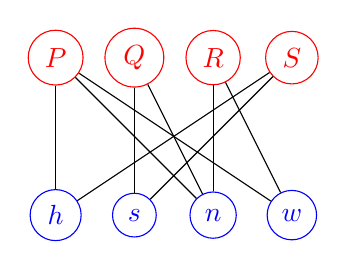
\begin{tikzpicture}
								\node[circle, draw, blue] (h) at (0, 0) {\(h\)};
								\node[circle, draw, blue] (s) at (1, 0) {\(s\)};
								\node[circle, draw, blue] (n) at (2, 0) {\(n\)};
								\node[circle, draw, blue] (w) at (3, 0) {\(w\)};
								\node[circle, draw, red] (P) at (0, 2) {\(P\)};
								\node[circle, draw, red] (Q) at (1, 2) {\(Q\)};
								\node[circle, draw, red] (R) at (2, 2) {\(R\)};
								\node[circle, draw, red] (S) at (3, 2) {\(S\)};
								\draw (P) -- (h);
								\draw (P) -- (n);
								\draw (P) -- (w);
								\draw (Q) -- (s);
								\draw (Q) -- (n);
								\draw (R) -- (n);
								\draw (R) -- (w);
								\draw (S) -- (h);
								\draw (S) -- (s);
							\end{tikzpicture}\]
					\end{tasks}
				\enumset{36}
				\item
					\begin{tasks}(3)
						\task
							\(|V| = n, |E| = \binom{n}{2}\)
						\task
							\(|V| = n, |E| = n\)
						\task
							\(|V| = n + 1, |E| = 2n\)
						\task
							\(|V| = m + n, |E| = mn\)
						\task
							\(|V| = 2^n, |E| = n2^{n - 1}\)
					\end{tasks}
				\enumset{52}
				\item
					why
			\end{enumerate}
		\subsection{Representing Graphs and Graph Isomorphism}
			\begin{enumerate}
				\item
					\[\begin{array}{|c|l|}\hline
						\text{Vertex} & \text{Adjacent Vertices} \\\hline
						a & b, c, d \\
						b & a, d\\
						c & a, d \\
						d & a, b, c \\\hline
					\end{array}\]
				\enumset{2}
				\item
					\[\begin{array}{|c|l|}\hline
						\text{Vertex} & \text{Terminal Vertices} \\\hline
						a & a, b, c, d \\
						b & d \\
						c & a, b \\
						d & b, c, d \\\hline
					\end{array}\]
				\enumset{4}
				\item
					\[\kbordermatrix{
								& a & b & c & d \\
								a & 0 & 1 & 1 & 1 \\
								b & 1 & 0 & 0 & 1 \\
								c & 1 & 0 & 0 & 1 \\
								d & 1 & 1 & 1 & 0
					}\]
				\enumset{6}
				\item
					\[\kbordermatrix{
								& a & b & c & d \\
								a & 1 & 1 & 1 & 1 \\
								b & 0 & 0 & 0 & 1 \\
								c & 1 & 1 & 0 & 0 \\
								d & 0 & 1 & 1 & 1
					}\]
				\enumset{8}
					\begin{tasks}(3)
						\task
							\[\begin{bmatrix}
								0 & 1 & 1 & 1 \\
								1 & 0 & 1 & 1 \\
								1 & 1 & 0 & 1 \\
								1 & 1 & 1 & 0 
							\end{bmatrix}\]
						\task
							\[\begin{bmatrix}
								0 & 1 & 1 & 1 & 1 \\
								1 & 0 & 0 & 0 & 0 \\
								1 & 0 & 0 & 0 & 0 \\
								1 & 0 & 0 & 0 & 0 \\
								1 & 0 & 0 & 0 & 0 
							\end{bmatrix}\]
						\task
							\[\begin{bmatrix}
								0 & 0 & 1 & 1 & 1 \\
								0 & 0 & 1 & 1 & 1 \\
								1 & 1 & 0 & 0 & 0 \\
								1 & 1 & 0 & 0 & 0 \\
								1 & 1 & 0 & 0 & 0 
							\end{bmatrix}\]
						\task
							\[\begin{bmatrix}
								0 & 1 & 0 & 1 \\
								1 & 0 & 1 & 0 \\
								0 & 1 & 0 & 1 \\
								1 & 0 & 1 & 0
							\end{bmatrix}\]
						\task
							\[\begin{bmatrix}
								0 & 1 & 1 & 1 & 1 \\
								1 & 0 & 1 & 0 & 1 \\
								1 & 1 & 0 & 1 & 0 \\
								1 & 0 & 1 & 0 & 1 \\
								1 & 1 & 0 & 1 & 0
							\end{bmatrix}\]
						\task
							\[\begin{bmatrix}
								0 & 1 & 1 & 0 & 1 & 0 & 0 & 0 \\
								1 & 0 & 0 & 1 & 0 & 1 & 0 & 0 \\
								1 & 0 & 0 & 1 & 0 & 0 & 1 & 0 \\
								0 & 1 & 1 & 0 & 0 & 0 & 0 & 1 \\
								1 & 0 & 0 & 0 & 0 & 1 & 1 & 0 \\
								0 & 1 & 0 & 0 & 1 & 0 & 0 & 1 \\
								0 & 0 & 1 & 0 & 1 & 0 & 0 & 1 \\
								0 & 0 & 0 & 1 & 0 & 1 & 1 & 0
							\end{bmatrix}\]
					\end{tasks}
				\enumset{10}
				\item
					\[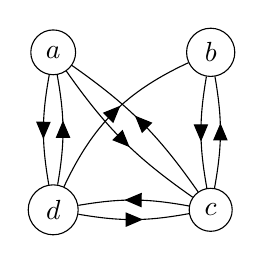
\begin{tikzpicture}[
							    midarr/.style 2 args={
							        decoration={             
							            markings, 
							            mark=at position 0.5 with {\arrow[xshift=3.333pt]{triangle 45}, \node[#1] {#2};}
							        },
							        postaction={decorate}
							    }
							]
						\node[circle, draw] (a) at (0, 2) {\(a\)};
						\node[circle, draw] (b) at (2, 2) {\(b\)};
						\node[circle, draw] (c) at (2, 0) {\(c\)};
						\node[circle, draw] (d) at (0, 0) {\(d\)};
						\draw[midarr] (a) to[bend right = 10] (c);
						\draw[midarr] (a) to[bend right = 10] (d);
						\draw[midarr] (b) to[bend right = 10] (c);
						\draw[midarr] (c) to[bend right = 10] (a);
						\draw[midarr] (c) to[bend right = 10] (b);
						\draw[midarr] (c) to[bend right = 10] (d);
						\draw[midarr] (d) to[bend right = 10] (a);
						\draw[midarr] (d) to[bend left = 20] (b);
						\draw[midarr] (d) to[bend right = 10] (c);
					\end{tikzpicture}\]
				\enumset{12}
				\item
					\[\kbordermatrix{
						& a & b & c & d \\
						a & 0 & 0 & 1 & 0 \\
						b & 0 & 0 & 1 & 2 \\
						c & 1 & 1 & 0 & 1 \\
						d & 0 & 2 & 1 & 0
					}\]
				\enumset{14}
				\item
					\[\kbordermatrix{
						& a & b & c & d \\
						a & 1 & 0 & 2 & 1 \\
						b & 0 & 1 & 1 & 2 \\
						c & 2 & 1 & 1 & 0 \\
						d & 1 & 2 & 0 & 1
					}\]
				\enumset{16}
				\item
					\[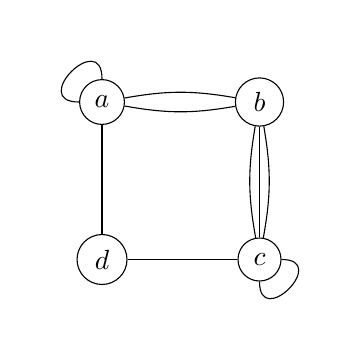
\begin{tikzpicture}
						\node[circle, draw] (a) at (0, 2) {\(a\)};
						\node[circle, draw] (b) at (2, 2) {\(b\)};
						\node[circle, draw] (c) at (2, 0) {\(c\)};
						\node[circle, draw] (d) at (0, 0) {\(d\)};
						\draw (a) to[out = 180, in = 90, looseness = 4] (a);
						\draw (a) to[bend right = 10] (b);
						\draw (a) to[bend left = 10] (b);
						\draw (a) to (d);
						\draw (b) to (c);
						\draw (b) to[bend left = 10] (c);
						\draw (b) to[bend right = 10] (c);
						\draw (c) to[out = 270, in = 360, looseness = 4] (c);
						\draw (c) to (d);
					\end{tikzpicture}\]
				\enumset{18}
				\item
					\[\kbordermatrix{
						& a & b & c & d \\
						a & 0 & 1 & 0 & 0 \\
						b & 0 & 1 & 1 & 0 \\
						c & 0 & 1 & 1 & 1 \\
						d & 1 & 0 & 0 & 0
					}\]
				\enumset{20}
				\item
					\[\kbordermatrix{
						& a & b & c & d \\
						a & 1 & 1 & 2 & 1 \\
						b & 1 & 0 & 0 & 2 \\
						c & 1 & 0 & 1 & 1 \\
						d & 0 & 2 & 1 & 0
					}\]
				\enumset{22}
				\item
					\[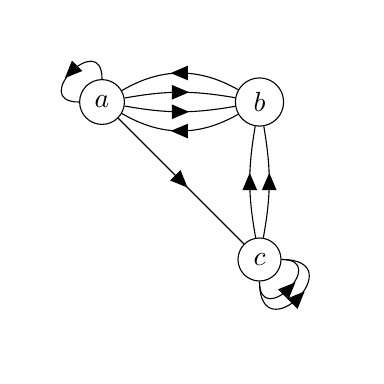
\begin{tikzpicture}[
						    midarr/.style 2 args={
						        decoration={             
						            markings, 
						            mark=at position 0.5 with {\arrow[xshift=3.333pt]{triangle 45}, \node[#1] {#2};}
						        },
						        postaction={decorate}
							}
						]
						\node[circle, draw] (a) at (0, 2) {\(a\)};
						\node[circle, draw] (b) at (2, 2) {\(b\)};
						\node[circle, draw] (c) at (2, 0) {\(c\)};
						\draw[midarr] (a) to[out = 90, in = 180, looseness = 4] (a);
						\draw[midarr] (a) to[bend right = 10] (b);
						\draw[midarr] (a) to[bend left = 10] (b);
						\draw[midarr] (a) to (c);
						\draw[midarr] (b) to[bend right = 30] (a);
						\draw[midarr] (b) to[bend left = 30] (a);
						\draw[midarr] (c) to[bend right = 10] (b);
						\draw[midarr] (c) to[bend left = 10] (b);
						\draw[midarr] (c) to[out = 270, in = 360, looseness = 4] (c);
						\draw[midarr] (c) to[out = 270, in = 360, looseness = 6] (c);
					\end{tikzpicture}\]
				\enumset{30}
				\item
					\[
						\mathbf{M}_{13} = \kbordermatrix{
								\\
								a & 1 & 0 & 0 & 0 & 0 \\
								b & 0 & 1 & 1 & 1 & 0 \\
								c & 1 & 1 & 1 & 1 & 1 \\
								d & 0 & 0 & 0 & 0 & 1
							} \qquad
						\mathbf{M}_{14} = \kbordermatrix{
								\\
								a & 1 & 1 & 1 & 1 & 0 & 0 & 0 & 0 \\
								b & 1 & 1 & 1 & 0 & 1 & 0 & 0 & 0 \\
								c & 0 & 0 & 0 & 0 & 1 & 1 & 1 & 1 \\
								d & 0 & 0 & 0 & 1 & 0 & 1 & 1 & 1
							}
					\]
					\[
						\mathbf{M}_{15} = \kbordermatrix{
								\\
								a & 1 & 1  & 1 & 1 & 0 & 0 & 0 & 0 & 0 & 0 \\
								b & 0 & 0 & 0 & 0 & 1 & 1 & 1 & 1 & 0 & 0 \\
								c & 0 & 1 & 1 & 0 & 0 & 1 & 0 & 0 & 1 & 0 \\
								d & 0 & 0 & 0 & 1 & 0 & 0 & 1 & 1 & 0 & 1
							}
					\] 
				\enumset{32}
				\item
					For an undirected graph, the sum of the entries in a column of the adjacency matrix is the number of edges that are connected to that column's vertex (loops only being counted once). For a digraph, it is the in-degree of the vertex.
				\enumset{34}
				\item
					For an undirected graph, the sum of the values of a column in the incidence matrix is equal to the number of nodes that the column's edge is incident to. This can only be 1 (if the edge is a loop) or 2.
				\item
					\begin{tasks}(2)
						\task
							\[\begin{bmatrix}
								1 & 1 & \cdots & 1 \\
								1 & 1 & \cdots & 1 \\
								\vdots & \vdots & & \vdots \\
								1 & 1 & \cdots & 1
							\end{bmatrix}\]
						\task
							\[\begin{bmatrix}
								0 & 1 & 0 & \cdots & 0 & 1 \\
								1 & 0 & 1 & \cdots & 0 & 0 \\
								0 & 1 & 0 & \cdots & 0 & 0 \\
								\vdots & \vdots & \vdots & & \vdots & \vdots \\
								1 & 0 & 0 & \cdots & 1 & 0
							\end{bmatrix}\]
						\task
							\[\begin{bmatrix}
								1 & 1 & 1 & \cdots & 1 & 1 \\
								1 & 0 & 1 & 0 & \cdots & 0 & 1 \\
								1 & 1 & 0 & 1 & \cdots & 0 & 0 \\
								1 & 0 & 1 & 0 & \cdots & 0 & 0 \\
								\vdots & \vdots & \vdots & & \vdots & \vdots \\
								1 & 0 & 0 & \cdots & 1 & 0
							\end{bmatrix}\]
						\task
							\[\begin{bmatrix}
								0 & \cdots & 1 \\
								\vdots & & \vdots \\
								1 & \cdots & 0	
							\end{bmatrix}\]
					\end{tasks}
				\item
					\begin{tasks}(2)
						\task
							\[\begin{bmatrix}
								1 & 1 & \cdots & 1 & 0 & \cdots & 0 \\
								1 & 0 & \cdots & 0 & 1 & \cdots & 0 \\
								0 & 1 & \cdots & 0 & 1 & \cdots & 0 \\
								\vdots & \vdots & & \vdots & \vdots & & \vdots \\
								0 & 0 & \cdots & 0 & 0 & \cdots & 1 \\
								0 & 0 & \cdots & 1 & 0 & \cdots & 1
							\end{bmatrix}\]
						\task
							\[\begin{bmatrix}
								1 & 0 & \cdots & 0 & 1 \\
								1 & 1 & \cdots & 0 & 0 \\
								0 & 1 & \cdots & 0 & 0 \\
								\vdots & \vdots & & \vdots & \vdots \\
								0 & 0 & \cdots & 1 & 0 \\
								0 & 0 & \cdots & 1 & 1
							\end{bmatrix}\]
						\task
							\[\begin{bmatrix}
								0 & 0 & \cdots & \cdots & 0 & 1 & 1 & \cdots & 1 \\
								1 & 0 & \cdots & 0 & 1 & 1 & 0 & \cdots & 0 \\
								1 & 1 & \cdots & 0 & 0  & 0 & 1 & \cdots & 0 \\
								0 & 1 & \cdots & 0 & 0  & \vdots & \vdots & & \vdots \\
								\vdots & \vdots & & \vdots & \vdots & \vdots & \vdots & & \vdots \\
								0 & 0 & \cdots & 1 & 0 & \vdots & \vdots & & \vdots \\
								0 & 0 & \cdots & 1 & 1 & 0 & 0 & \cdots & 1
							\end{bmatrix}\]
						\task
							\[\begin{bmatrix}
								1 & 1 & \cdots & 1 & 0 & \cdots & 0 \\
								0 & 0 & \cdots & 0 & 1 & \cdots & 0 \\
								\vdots & \vdots & & \vdots & \vdots & & \vdots \\
								0 & 0 & \cdots & 0 & 0 & \cdots & 1 \\
								1 & 0 & \cdots & 0 & 1 & \cdots & 0 \\
								0 & 1 & \cdots & 0 & 0 & \cdots & 1 \\
								\vdots & \vdots & & \vdots & \vdots & & \vdots \\
								0 & 0 & \cdots & 1 & 0 & \cdots & 0
							\end{bmatrix}\]
					\end{tasks}
				\enumset{38}
				\item
					\[\begin{array}{|c|*{5}{c}|}\hline
						v & u_1 & u_2 & u_3 & u_4 & u_5 \\\hline
						f(v) & v_1 & v_3 & v_2 & v_5 & v_3 \\\hline
					\end{array}\]
				\enumset{40}
				\item
					\[\begin{array}{|c|*{7}{c}|}\hline
						v & u_1 & u_2 & u_3 & u_4 & u_5 & u_6 & u_7 \\\hline
						f(v) & v_1 & v_3 & v_5 & v_7 & v_2 & v_4 & v_6  \\\hline
					\end{array}\]
				\enumset{42}
				\item
					\[\begin{array}{|c|*{6}{c}|}\hline
						v & u_1 & u_2 & u_3 & u_4 & u_5 & u_6 \\\hline
						f(v) & v_5 & v_2 & v_3 & v_6 & v_4 & v_1 \\\hline
					\end{array}\]
				\enumset{44}
				\item
					\(u_5\) is connected to exactly 2 other nodes, both of which are of degree \(3\). There is no node in the second graph that has this property. The graphs are therefore nonisomorphic.
				\enumset{46}
				\item
					\[\begin{array}{|c|*{10}{c}|}\hline
						v & u_1 & u_2 & u_3 & u_4 & u_5 & u_6 & u_7 & u_8 & u_9 & u_{10} \\\hline
						f(v) & v_6 & v_5 & v_8 & v_{10} & v_7 & v_3 & v_9 & v_2 & v_4 & v_1 \\\hline
					\end{array}\]
				\enumset{62}
				\item
					\begin{tasks}(2)
						\task
							\[
								\kbordermatrix{
									& v_1 & v_2 & v_3 \\
									v_1 & 0 & 0 & 1 \\
									v_2 & 0 & 0 & 1 \\
									v_3 & 1 & 1 & 0
								}	\implies \kbordermatrix{
									& v_3 & v_1 & v_2 \\
									v_3 & 0 & 1 & 1 \\
									v_1 & 1 & 0 & 0 \\
									v_2 & 1 & 0 & 0
								}
							\]
							Yes
						\task
							No, as there is no row in the first matrix with only 1 1.
						\task
							No, as there is no row in the first matrix with only 1 1.
					\end{tasks}
				\enumset{66}
				\item
					\[\begin{array}{|c|*{4}{c}|}\hline
						v & u_1 & u_2 & u_3 & u_4 \\\hline
						f(v) & v_3 & v_4 & v_2 & v_1
					\end{array}\]
				\enumset{68}
				\item
					\[\begin{array}{|c|*{4}{c}|}\hline
						v & u_1 & u_2 & u_3 & u_4 \\\hline
						f(v) & v_3 & v_4 & v_2 & v_1 \\\hline
					\end{array}\]
			\end{enumerate}
		\setcounter{subsection}{4}
		\subsection{Euler and Hamilton Paths}
			\begin{enumerate}
				\item
					\(a\), \(b\) and \(c\) are all of degree 3, which means that 3 nodes are of odd degree, so the graph has neither an Euler path or circuit.
				\enumset{2}
				\item
					\(a\) and \(d\) are of odd degree while every other is of even degree, so an Euler path may exist. Such a path is \((a, e, c, e, b, e, d, b, a, c, d)\).
				\enumset{4}
				\item
					Every vertex is of even degree, so the graph may have an Euler circuit. Such a circuit is \((a, e, a, e, c, d, c, b, e, d, b, a)\).
				\enumset{6}
				\item
					Every vertex is of even degree, so the graph may have an Euler circuit. Such a circuit is \((a, i h, g, d, e, f, g, c, e, h, d, c, a, b, i, c, b, h, a)\).
				\enumset{12}
				\item
					This image can be drawn in a single stroke by treating the intersections of edges as nodes. \\
				\enumset{14}
				\item
					This image cannot be drawn in a single stroke. \\
				\enumset{18}
				\item
					\[\begin{array}{|c|*{4}{c}|}\hline
						v & a & b & c & d \\\hline
						\deg^-v & 1 & 3 & 1 & 2 \\\hline
						\deg^+v & 2 & 1 & 2 & 2 \\\hline
					\end{array}\]
					\(\deg^-v\) is not always equal to \(\deg^+v\), so an Euler circuit may not exist. \(\deg^+a - \deg^-a = \deg^+c - \deg^-c = 1\), so an Euler path may not exist either. \\
				\enumset{20}
				\item
					An Euler path exists: \(a, d, e, d, b, a, e, c, e, b, c, b, e\).
				\enumset{22}
				\item
					\[\begin{array}{|c|*{12}{c}|}\hline
						v & a & b & c & d & e & f & g & h & i & j & k & l \\\hline
						\deg^-v & 1 & 2 & 1 & 1 & 2 & 1 & 2 & 2 & 2 & 1 & 1 & 1 \\\hline
						\deg^+v & 1 & 1 & 1 & 2 & 2 & 2 & 1 & 2 & 1 & 1 & 2 & 1 \\\hline
					\end{array}\]
					\(\deg^-v\) is not always equal to \(\deg^+v\), so an Euler circuit may not exist. \(\deg^+d - \deg^-d = \deg^+f - \deg^-f = 1\), so an Euler path may not exist either. \\
				\enumset{25}
				\item
					\begin{tasks}(2)
						\task	
					\end{tasks}

			\end{enumerate}
\end{document}

